%\title{EMC LaTeX Portrait Poster Template}
%%%%%%%%%%%%%%%%%%%%%%%%%%%%%%%%%%%%%%%%%
% a1poster Portrait Poster
% LaTeX Template
% Version 2.0 (22/06/16)
%
% The a1poster class was created by:
% Joe Rowing (JoeRowing@exeterms.ac.uk)
% 
% This template has been produced by:
% Joe Rowing at Exeter Mathematics School
%
% License:
% CC BY-NC-SA 3.0 (http://creativecommons.org/licenses/by-nc-sa/3.0/)
%
%%%%%%%%%%%%%%%%%%%%%%%%%%%%%%%%%%%%%%%%%

%----------------------------------------------------------------------------------------
%   PACKAGES AND OTHER DOCUMENT CONFIGURATIONS
%----------------------------------------------------------------------------------------

\documentclass[a1,portrait]{a1poster}

\usepackage{multicol} % This is so we can have multiple columns of text side-by-side
\columnsep=50pt % This is the amount of white space between the columns in the poster
\columnseprule=0.01pt % This is the thickness of the black line between the columns in the poster
\usepackage[svgnames]{xcolor} % Specify colors by their 'svgnames', for a full list of all colors available see here: http://www.latextemplates.com/svgnames-colors

\usepackage{times} % Use the times font
\usepackage{pgfplots}
\usepackage{tikz}
\usepackage{graphicx} % Required for including images
% \graphicspath{{assets/}} % Location of the graphics files
\usepackage{booktabs} % Top and bottom rules for table
\usepackage[font=small,labelfont=bf]{caption} % Required for specifying captions to tables and figures
\usepackage{amsfonts, amsmath, amsthm, amssymb} % For math fonts, symbols and environments
\usepackage{wrapfig} % Allows wrapping text around tables and figures

\begin{document}

%----------------------------------------------------------------------------------------
%   POSTER HEADER 
% The header is divided into two boxes:
% The first is 75% wide and houses the title, subtitle, names, university/organization and contact information
% The second is 25% wide and houses the EMS Logo
% 
%----------------------------------------------------------------------------------------

\begin{minipage}[b]{0.6\linewidth}
\Huge \color{DarkRed} \textbf{Neural Networks} \color{Black}
\\ % Title
% \huge\textit{With a subtitle here}\\[1cm] % Subtitle
\large \textbf{Oliver Temple}\\[0.5cm] % Author(s)
\large Exeter Mathematics School\\[0.2cm] % University/organization
\texttt{olivertemple@exe-coll.ac.uk}\\
\end{minipage}
%
\begin{minipage}[b]{0.4\linewidth}

\includegraphics[width=15cm]{emsnew.PNG}\\
\end{minipage}

\vspace{.5cm} % A bit of extra whitespace between the header and poster content

%----------------------------------------------------------------------------------------

\begin{multicols}{2} % This is how many columns your poster will be broken into, by convention a portrait poster is generally split into 2 or 3 columns

%----------------------------------------------------------------------------------------
%   ABSTRACT

%An abstract is a brief summary of a research article, thesis, review, conference proceeding or any in-depth analysis of a particular subject and is often used to help the reader quickly ascertain the paper's purpose
%----------------------------------------------------------------------------------------

\color{DarkRed} % Colour for the abstract

\begin{abstract}

    Now commonplace in todays world, neural networks are becoming increasingly popular, but what actually are they, and how do they work? This project will explore the basic concepts behind neural networks, how they are used in the real world and how the most simple neural networks work at a low level. The project will conclude by exploring how to code a neural network from scratch to recognize hand written digits from 0-9.

    Neural networks are complex computational models that have many uses. There are many different types of neural networks that each have their own pros and cons, making them suited for specific tasks, from computer vision, to classification and prediction. The structure of neural networks can vary dramatically for different models, allowing for a wide range of applications. Activation functions, loss functions, number of layers and neurons are just a few of the structure parameters that can be changed to create a neural network that suits the problem.

\end{abstract}

%----------------------------------------------------------------------------------------
%   INTRODUCTION

%Avoid using technical definitions unless absolutely necessary. The introduction section is here to introduce your issue, so be sure to not bore your readers right away with excessive information. You can even include graphics if they will help the viewer understand the work that you have done.
%----------------------------------------------------------------------------------------

\color{Black} % color for the introduction

\section*{Introduction}
Neural networks are complex computational models used to perform a wide range of tasks. This project looks into what neural networks are, what they are used for and how to code a simple neural network to recognize hand written digits from 0 to 9, using the MNIST dataset to train the network.

%----------------------------------------------------------------------------------------
%   OBJECTIVES
%----------------------------------------------------------------------------------------

\color{Black} % DarkSlateGray color for the rest of the content

\section*{Main Objectives}

\begin{enumerate}
\item Explore the different types of neural network models.
\item Explore the uses of different types of neural network models.
\item Explore how a neural network works from a high level.
\item Explore how to use a neural network to classify handwritten digits from 0-9.
\item Code a neural network to recognize handwritten digits form 0-9.
\end{enumerate}

%----------------------------------------------------------------------------------------
%   MATERIALS AND METHODS

% In this section you will cover the materials and methods (shocking!) that you used in your research process. Feel free to include any images, charts, or graphs here that will help the viewer better understand your process. Also, don’t forget to provide a rationale to explain why you chose these methods! This is just as important as the steps you took
%----------------------------------------------------------------------------------------

\section*{Types of Neural Networks}
There are many different types of neural networks, each with their own advantages and disadvantages that make them best suited for specific tasks. The most common types of neural networks are:
\begin{itemize}
    \item Perceptron
    \item Feed Forward Neural Network
    \item Multi-layer Perceptron
    \item Convolutional Neural Network
\end{itemize}

\subsection*{Perceptron}
\begin{wrapfigure}{R}{0.2\textwidth}
    \centering
    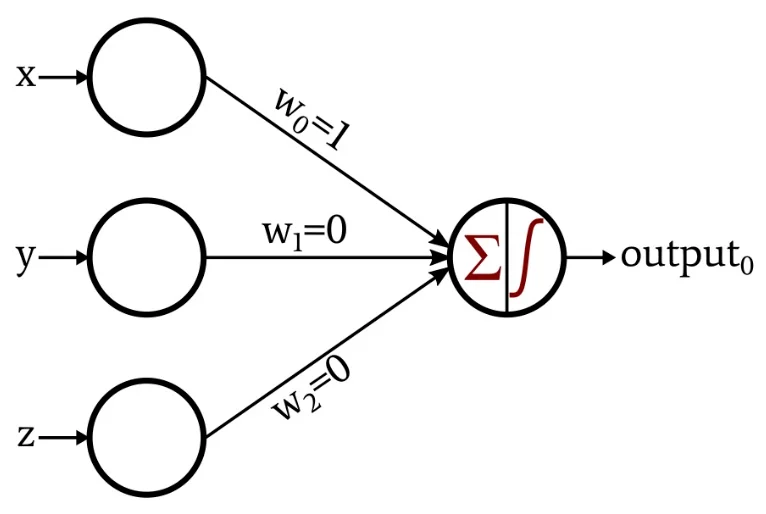
\includegraphics[width=0.2\textwidth]{assets/perceptron.png}
    \caption{Perceptron}
    \label{fig:perceptron}
\end{wrapfigure}
The perceptron is the simplest component of a neural network, often referred to as a neuron. It accepts weighted inputs and outputs a single output. The output of a perceptron is calculated by taking the vector dot product of the weights and the inputs:
\begin{equation}
    \textbf{y} = \textbf{W}\cdot\textbf{x} + b
    \label{eq:perceptron}
\end{equation}
Where $\textbf{y}$ is the output, $\textbf{W}$ is a vector of the weights, $\textbf{x}$ is a vector of the inputs, and $b$ is the bias.

\subsection*{Feed Forward Neural Network}
A feed forward neural network is constructed from a set of interconnected layers. Each neuron in a layer is connected to all of the neurons in the previous layer, and the output of each layer fed forward into the next layer and used as the input. The data only travels forwards through the network, making them useful only for linear classification. Each connection has a weight, and each neuron has a bias, which are used to calculate the output of the network. The output is calculated by: 
\begin{equation}
    \textbf{y}_n=\sigma{(\textbf{W}_n\cdot\textbf{y}_{n-1} + \textbf{b}_n)}
    \label{eq:feed-forward}
\end{equation}
Where $\textbf{y}_n$ is the output vector of the nth layer, $\textbf{W}_n$ is the weight matrix of the nth layer, $\textbf{y}_{n-1}$ is the output vector of the previous layer, $\textbf{b}_n$ is the bias vector of the nth layer, and $\sigma$ is the activation function.
\begin{wrapfigure}{R}{0.2\textwidth}
    \centering
    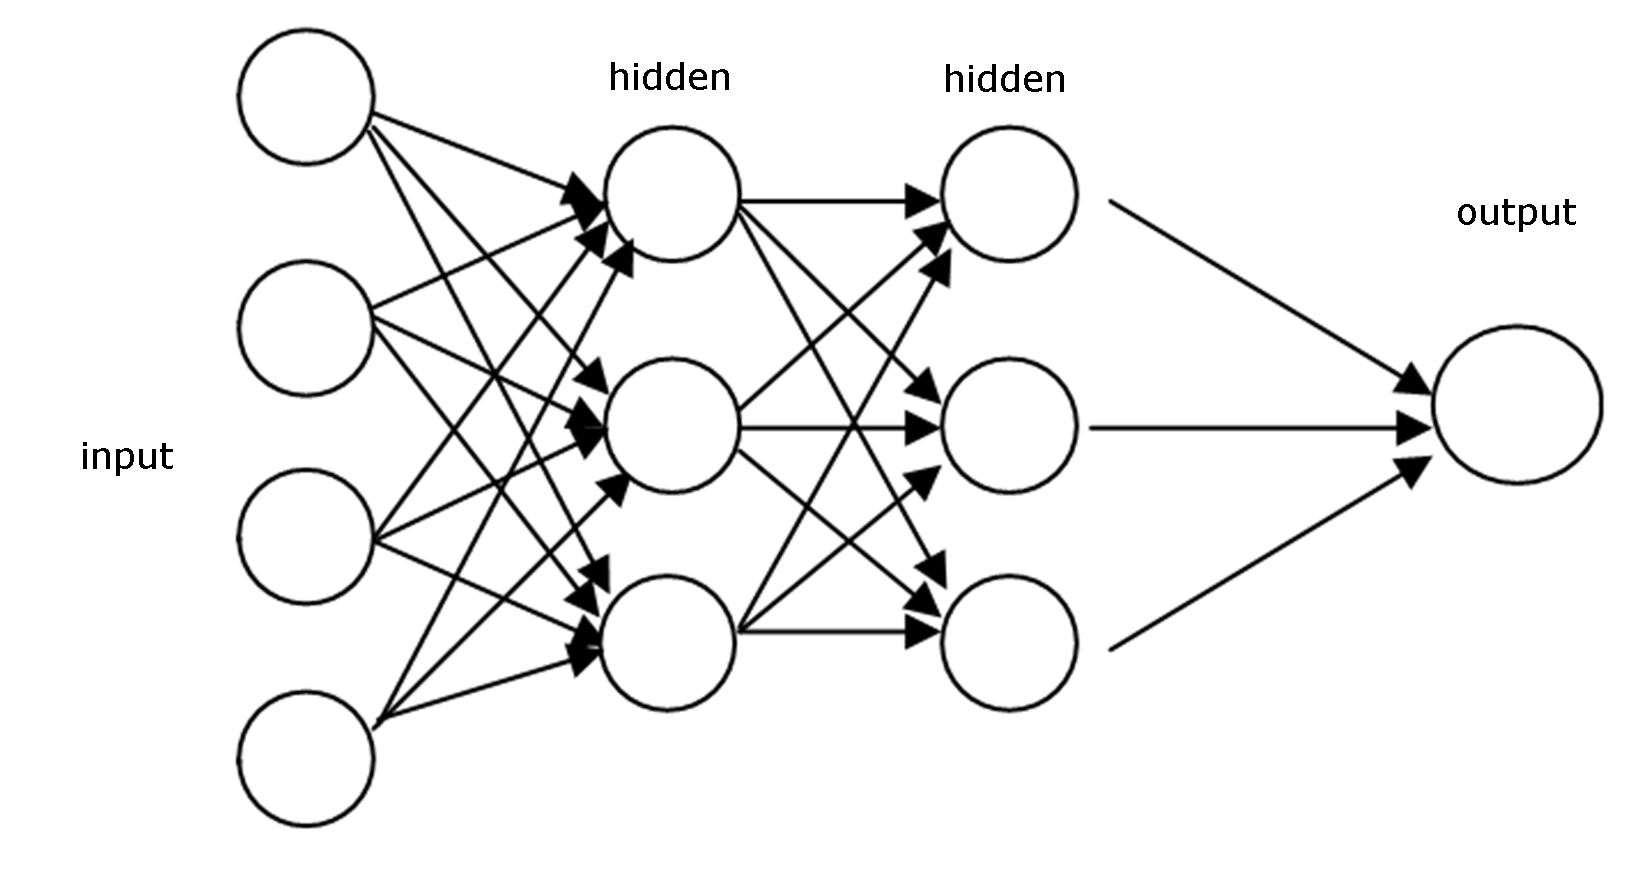
\includegraphics[width=0.2\textwidth]{assets/feed forward.png}
    \caption{Feed Forward Neural Network}
    \label{fig:feed-forward}
\end{wrapfigure}
\subsection*{Multi-layer Perceptron}
A multi-layer perceptron is much like a feed forward neural network, in the sense that it is made up of interconnected layers of neurons, however, the data can travel both forwards and backwards through the network allowing for the network to be trained. The process in which the data travels backwards through the network is called back propagation and involves the altering of the weights and biases of the network. The output of the network is calculated the same as a feed forward network (See equation \ref{eq:feed-forward}).

\subsection*{Convolutional Neural Network}
\begin{wrapfigure}{L}{0.2\textwidth}
    \centering
    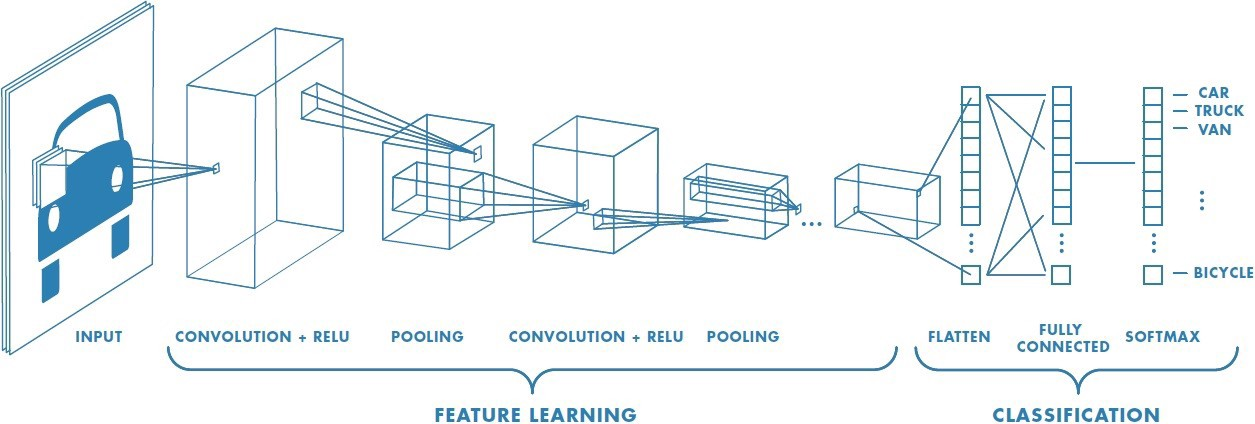
\includegraphics[width=0.2\textwidth]{assets/convolutional.jpeg}
    \caption{Convolutional Neural Network}
    \label{fig:convolutional}
\end{wrapfigure}
A convolutional neural network is often used for image recognition and contains a three dimensional arrangement of neurons. Each neuron on the first layer only processes information from a small part of the field of view. We will not be using a convolutional neural network in this project, as a multi-layer perceptron will suffice.
\subsection*{Other Models}
There are many other models beyond these that each have their own uses. The ones outlined here are some of the most common network models as well as one that is specialized for image recognition.

%------------------------------------------------
\section*{How Neural Networks Work}
At its core, a neural network is a collection of interconnected neurons formed into layers. Each neuron has its own bias, and each connection has a weight, which are used to calculate the output of the network. For our model for classifying handwritten digits from 0-9, we will be using a multilayer perceptron.
\subsection*{Structure}
\begin{wrapfigure}{L}{0.15\textwidth}
    \centering
    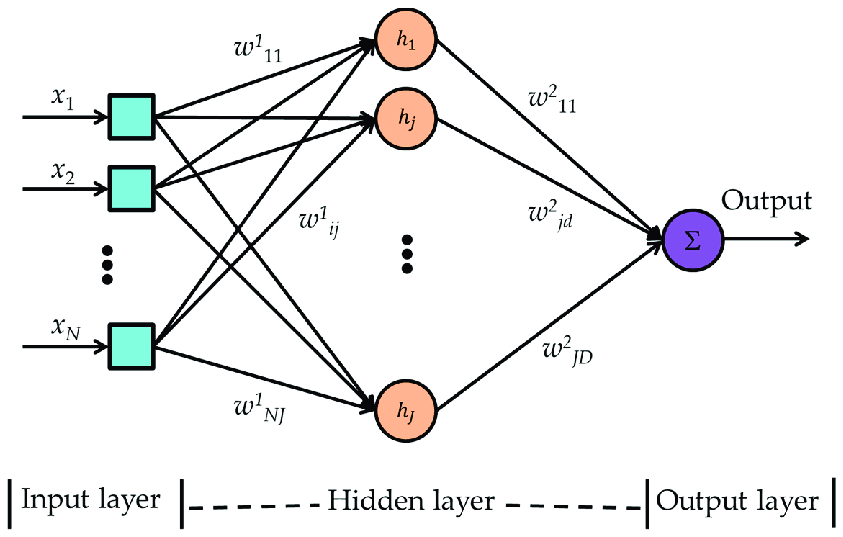
\includegraphics[width=0.15\textwidth]{assets/multilayer perceptron.png}
    \caption{Multi-layer Perceptron Structure}
    \label{fig:structure}
\end{wrapfigure}
The neuron with the highest output in the final layer will be the prediction of the network.
The structure of the network is the first thing that must be defined. The input layer must consist of the same number of neurons as there are data points, and the output layer must consist of the same number of neurons as there are classification labels. There can be any number of hidden layers, which can have any number of neurons. The size and number of hidden layers should be varied to determine what sizes give the best results for the problem. 

\subsection*{Forward Propagation}
Forward propagation is when the data is fed forward through the network to get a prediction. To calculate the output, we take the weighted sum of the inputs, add the bias add pass it though the activation function (See equation \ref{eq:feed-forward}).
\\\\
\subsection*{Activation Functions}
\begin{wrapfigure}{R}{0.2\textwidth}
    \centering
    \begin{tikzpicture}
        \begin{axis}[axis x line=bottom, axis y line=middle, xmin=-6, xmax=6]
        \addplot[color=red]{1/(1+exp(-x))};
        \end{axis}
    \end{tikzpicture}
    \caption{Sigmoid Function}
    \label{fig:sigmoid}
\end{wrapfigure}
The activation function is applied to the output of each neuron before it is inputted into the next layer. The purpose is to prevent the input being too high or too low, and to add some non-linearity to the network. There are many different activations to choose from and we will be using the sigmoid function, due to the simplicity of the problem not requiring a complex activation function.
\begin{equation}
    \sigma(x)=\frac{1}{1+e^{-x}}
    \label{eq:sigmoid}
\end{equation}

\subsection*{Loss Functions}
The loss function is used to calculate how good a network is. In order to calculate the loss we need the output of our network, and the expected output. Similar to activation functions, there are many loss functions to choose from, but we will be using the mean squared error (MSE) loss function due to the simplicity of the problem.
\begin{equation}
    \texttt{MSE} = \frac{1}{n}\sum_{i=1}^{n}(\hat{y}_i - y_i)^2
    \label{eq:mse}
\end{equation}
Where $n$ is the number of samples, $y_i$ is the desired output of the network, and $\hat{y}_i$ is the actual output of the network.
\subsection*{Back Propagation}
\begin{wrapfigure}{L}{0.2\textwidth}
    \centering
    \begin{tikzpicture}
        \begin{axis}[axis x line=middle, axis y line=middle, xlabel={Weight}, ylabel={Loss}]
        \addplot[color=red]{x*x};
        \end{axis}
    \end{tikzpicture}
    \caption{Example of Loss against Weight}
    \label{fig:loss-weight}
\end{wrapfigure}
Back propagation is the process in which the data moves backwards through the network, adjusting the weights and biases to minimize the loss function. To do so, the derivative of the loss function must first be calculated, as this will allow us to know whether to increase or decrease the weights and biases, and by how much.

For example, if a graph of loss against weight is plotted, as seen in Figure~\ref{fig:loss-weight}, the minimum of the function is calculated by using the derivative. However, as the loss function is usually in many more dimensions, the minimum cannot be calculated exactly and small steps towards the minimum are required.

When we have the derivative of the loss function, we know whether to increase or decrease the weights and biases due to the sign of the gradient. The weights and biases can be changed proportionally to the gradient to prevent missing the minimum of the function.

\subsection*{Training}
In order for a network to be used to classify data, it must first be trained. Before we can train the network, we must first initialize the weights and bias with small random values. Next, we must split our dataset into training data and testing data, so that once training has been completed we can test the model on unseen data to get an idea of how it would perform in the real world.  Training a network is done through the following process:
\begin{enumerate}
    \item Propagate all the values in the input layer thought the network (Forward Propagation).
    \item Update the weights and biases of the network using the loss function (Back Propagation).
    \item Repeat until the accuracy of the network is satisfactory.  
\end{enumerate}

\section*{Coding a neural network}
\subsection*{Data}
When training a neural network, one of the most important assets in the data that will be used to train the network. Any imperfections in the data, such as incorrect labels or biases will be reflected in the predictions of the network. For out model, we will be using the MNIST dataset, which is a large dataset of handwritten digits from 0-9.

\subsection*{Splitting the Data}
When creating a neural network, it is important to split the dataset into a training set and a testing set. This will allow us to test the network on unseen data. For our model we will use 50000 training samples and 10000 testing samples.

\subsection*{Defining the Model}
Before training the model, we have to define the structure. Our network will consist of layers of interconnected neurons, and when defining our model, we must decide how many layers we want and how many neurons should be in each layer. We also need to define our loss function and our activation function. We will be using the sigmoid function (equation~\ref{eq:sigmoid}) for our activation function, and the mean squared error (equation~\ref{eq:mse}) loss function. We also need to define the derivative of our loss function for back propagation. The derivative of the sigmoid function is:
\begin{equation}
    \sigma'(x) = x(1-x)
    \label{eq:sigmoid-prime}
\end{equation}
\subsubsection*{Layers}
The input layer will consist of 784 neurons, as the size of the input images is 28x28. We will be using one hidden layer of 350 neurons. The output layer will consist of 10 neurons, as there are only 10 possible outputs.

\subsection*{Training the Model}
\begin{wrapfigure}{L}{0.15\textwidth}
    \centering
    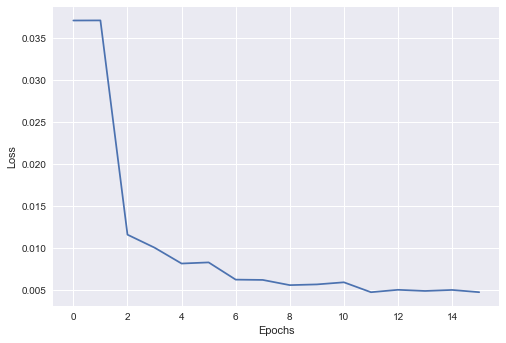
\includegraphics[width=0.15\textwidth]{assets/loss.png}
    \caption{Loss of network over epochs}
    \label{fig:loss-over-epochs}
\end{wrapfigure}
To train the model, the data is split up into equal sized batches. After a batch of data has been fed forward through the network, we will back propagate and adjust the weights and biases. Each batch is called a epoch. Training the network this way saves time, as back propagation can be computationally intensive. 

%----------------------------------------------------------------------------------------
%   RESULTS 

%It’s always a good idea to begin the Results section with an initial summary of your results. Don’t address your research question just yet; instead, just address the general aspects of the data you collected or the number of valid data obtained.

%In your next paragraph, you can discuss the relationship between the data and your research question. What exactly does your data mean? Be sure to include any graphics that can help show you data visually, as the readers can understand graphics more easily and quickly than blocks of text.

%Sometimes less is more. Be selective when deciding what images, charts, and graphs make it onto your poster! 

%Charts and graphs are usually more effective than tables, but whatever you choose to use, make sure everything is labeled clearly! A graph with missing labels or a table without a title will just leave the reader confused. Also, carefully consider what type of chart or graph will best show your results. K. Broman, professor of Biostatistics & Medical Informatics at the University of Wisconsin Madison has written a great article titled, “The Top Ten Worst Graphs.” (http://www.biostat.wisc.edu/~kbroman/topten_worstgraphs/)
%----------------------------------------------------------------------------------------

\section*{Results}
\begin{wrapfigure}{R}{0.2\textwidth}
    \centering
    
\includegraphics[width=0.2\textwidth]{assets/sample_predictions.png}
    \caption{Sample Predictions}
    \label{fig:sample-predictions}
\end{wrapfigure}
To calculate the accuracy of our trained model, we will feed every item in the testing dataset forward, keeping track of how many correct predictions there are. The accuracy of our model was 95.32\%. To get an idea of what our neural network is predicting, we will feed 9 random testing samples into it, draw them, and compare them to what was predicted. The images shown in figure~\ref{fig:sample-predictions} were fed into the network, and the predictions were 8, 5, 8, 9, 1, 9, 7, 2, 8 and the actual values were 5, 5, 8, 9, 1, 9, 7, 2, 8. In this sample, we get an accuracy of 88\%. This is lower, as only 9 samples were used.


%----------------------------------------------------------------------------------------
%   CONCLUSIONS
%In your conclusion section you want to briefly review your research questions and the results you obtain. You also should add why your results are interesting or significant. TIPS: Relate your results to other published research in the field. This will give your research more impact on your readers as well as show your professionalism in the study. You can also suggest continuing research that would build upon your current study.
%----------------------------------------------------------------------------------------

\color{FireBrick} %  colour for the conclusions to make them stand out

\section*{Conclusion}
To conclude, neural networks are complex models that are used for different tasks. There are many different types of neural networks that each have their own merits and downfalls, that are best for different tasks. Although it is possible to code neural networks from scratch, it is much easier and quicker to use a library, as they are very well optimized and already have complex loss and activation functions implemented, as well as many different types of neural network.

\color{Black} % Set the color back to DarkSlateGray for the rest of the content

%----------------------------------------------------------------------------------------
%   FORTHCOMING RESEARCH
%----------------------------------------------------------------------------------------

 %----------------------------------------------------------------------------------------
%   REFERENCES
%If you have an extremely extensive list of references, you may want to break it into 2 columns. 

% It is common to shrink the font of the References section if it becomes overbearing and long

%----------------------------------------------------------------------------------------
\begin{small}%Makes the text of the references section smaller
\begin{multicols}{2}%Makes the section two col
\nocite{*} % Print all references regardless of whether they were cited in the poster or not
\bibliographystyle{plain} % Plain referencing style
\bibliography{bibliography} % Use the example bibliography file sample.bib
\end{multicols}
\end{small}
%----------------------------------------------------------------------------------------
%   ACKNOWLEDGEMENTS
%You can acknowledge people who have helped you with your work, such as other members of your research group or your funding source. If there are any conflicts of interest regarding you and the work you have presented, be sure to include that here. It is always important to keep you and your work above reproach. Keep this section as short as possible. Fewer than 40 words is best.
%----------------------------------------------------------------------------------------

% \section*{Acknowledgements}

% Etiam fermentum, arcu ut gravida fringilla, dolor arcu laoreet justo, ut imperdiet urna arcu a arcu. Donec nec ante a dui tempus consectetur. Cras nisi turpis, dapibus sit amet mattis sed, laoreet.

%----------------------------------------------------------------------------------------
%	 CONTACT DETAILS
%A lot of posters include this section so the readers are able to contact the author later or read more about the research. You can include your email or website address, links to relevant resources, or even a QR code (What is a QR Code?) that viewers can scan to go directly to your website or a PDF version of your poster. If you choose to include this section, keep it very brief
%----------------------------------------------------------------------------------------
\section*{Contact Details}
Oliver Temple - olivertemple@exe-coll.ac.uk
\end{multicols}
\end{document}